\documentclass[12pt]{article}
%\usepackage[utf8]{inputenc}
%\documentclass[UTF8]{ctexart}
%\usepackage[UTF8, heading = false, scheme = plain]{ctex}
\usepackage{geometry}
%geometry{a4paper,scale=0.9}
\geometry{a4paper,left=1cm,right=1cm,top=1cm,bottom=2cm}
\usepackage{amsfonts}
\usepackage{color}
\usepackage{url}
%\usepackage{biblatex}
\usepackage{amsmath}
\usepackage{amssymb}
\usepackage{latexsym}
\usepackage{cite}
%\addbibresource{ref.bib}
%\bibliography{ref.bib}
\usepackage{caption}
\usepackage{graphicx, subfig}
\usepackage{float}
%\usepackage[fontset=ubuntu]{ctex}
%\usepackage{fontspec}
\usepackage{xeCJK}
%\usepackage[colorlinks,
%anchorcolor=black,
%citecolor=black]{hyperref}
%\setmainfont{SimSun}
\usepackage[section]{placeins}
\usepackage{enumitem}
\usepackage{framed}
\usepackage[framemethod=TikZ]{mdframed}
\usepackage{indentfirst}
\usepackage{setspace}%使用间距宏包
\linespread{1.5}
%\title{预备知识}
%\author{leolinuxer }
%\date{June 2020}

\title{财务相关}
%\author{leolinuxer }
%\date{June 2020}

\begin{document}
%\setlength{\parindent}{0pt}
\maketitle
\tableofcontents

参考书籍:《世界上最简单的会计书》

\section{基础知识}
\subsection{资产负债表}
存货(Inventory)是描述原材料、正在加工的在产品和准备出手的产成品的专业术语。

商品销售成本:产品生产过程中的所有支出;费用:企业经营中与产品生产不直接相关的其他支出;即剔除产品生产成本之外,企业经营所需要的花费。对于没有有形产品的公司(即服务类行业),这两类称为营业成本(或服务成本)和费用。

毛利 = 销售收入 - 商品销售成本

净利润(底线值) = 毛利 - 费用

资产负债表如下:
\begin{figure}[H]
    \centering
    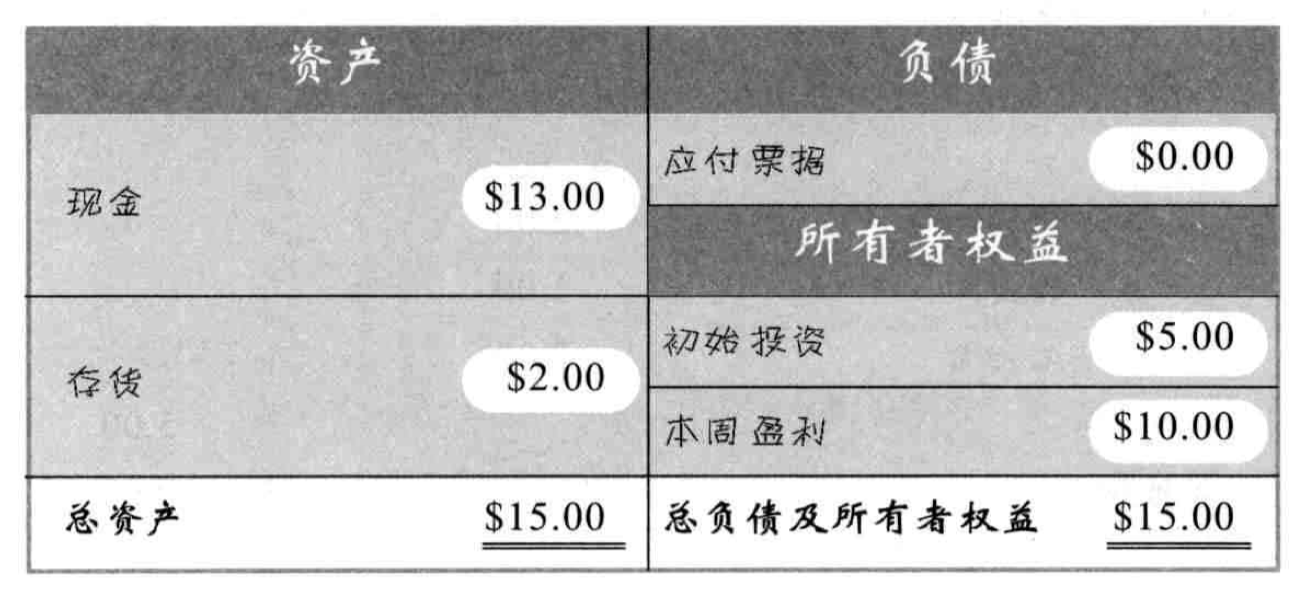
\includegraphics[width=1\textwidth]{fig/accounting_1.png}
\end{figure}

资产负债表的左边是资产,即我们所拥有的东西;

资产负债表的右边是负债(我们欠别人的)和所有者权益(你自己拥有的);

资产负债表的左右两边必须相等。所以:\textbf{资产 = 负债 + 所有者权益}。

资产负债表编制的目的就是在人(右边)和物(左边)建立一种联系。它表明了你在生意中所拥有的东西,以及这些东西与那些拥有它的人或对此有要求权的人们之间的关系。资产负债表展示的是瞬间的状况,就像一张快照。

\subsection{运营报表/利润表/损益表}
利润表就像一部电影,描述的是动态变化。

利润表将成本分为两部分:商品销售成本和费用。

利润表编制的目的,是记录销售收入减去销售成本而获得企业某段时期的毛利,然后再剔除所发生的的其他费用,从而得到净利润。

利润表如下:
\begin{figure}[H]
    \centering
    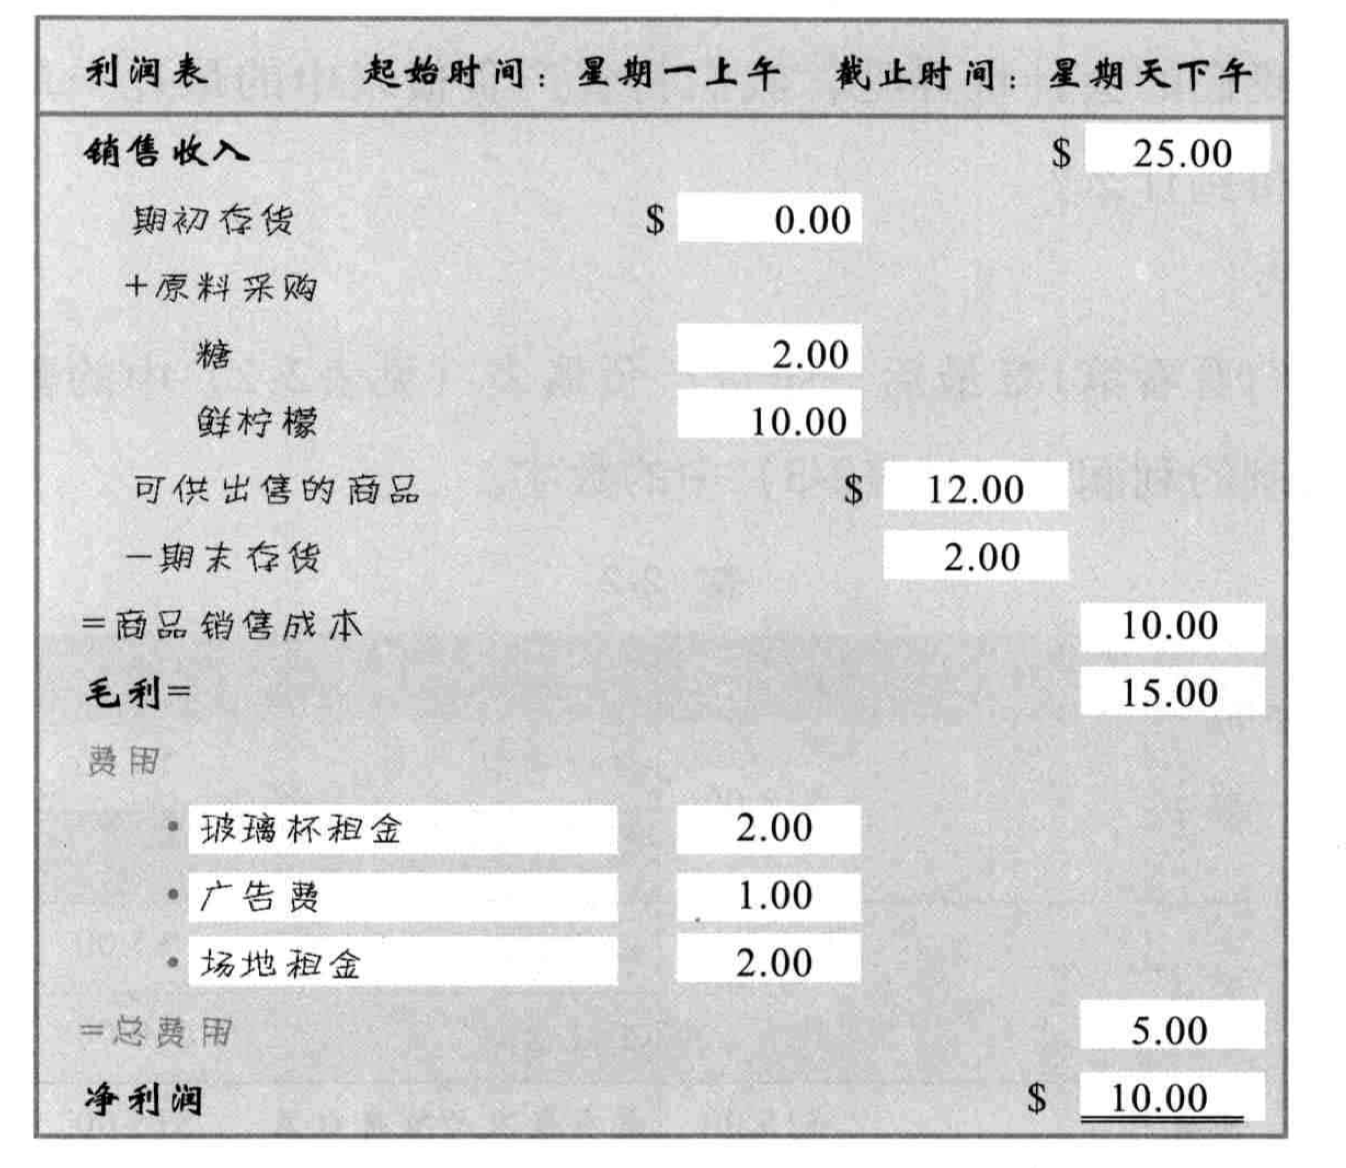
\includegraphics[width=1\textwidth]{fig/accounting_2.png}
\end{figure}

\subsection{资产负债表和利润表的关系}
\begin{itemize}
\setlength{\itemsep}{0pt}
\setlength{\parsep}{0pt}
\setlength{\parskip}{0pt}
    \item 净利润和盈利相等;
    \item 存货也一样;
\end{itemize}

为什么期末存货会同时出现在两张表中?因为我们没有使用它。期末存货不能算作销售成本,因为我们没有把它销售出去,所以在利润表中,我们从可供销售的商品中减掉它们;而在资产负债表中,因为我们没有卖掉它,它的价值仍然存在,我们仍旧拥有它。

每个会计周期的末期,会得到期末资产负债表,里面的存货代表期末存货;每个会计周期的初期,会得到期初资产负债表,里面的存货代表期初存货。期末存货会自动变为下期的期初存货。

是什么将期初资产负债表和期末资产负债表联系起来的?是利润表。

\subsection{一些术语}
留存收益:过去会计期间的累积盈利。

盈利可以用来做两件事,即把它们留在生意里或者把它们分给公司股东(给股东发放红利)。

增加了留存收益的资产负债表:
\begin{figure}[H]
    \centering
    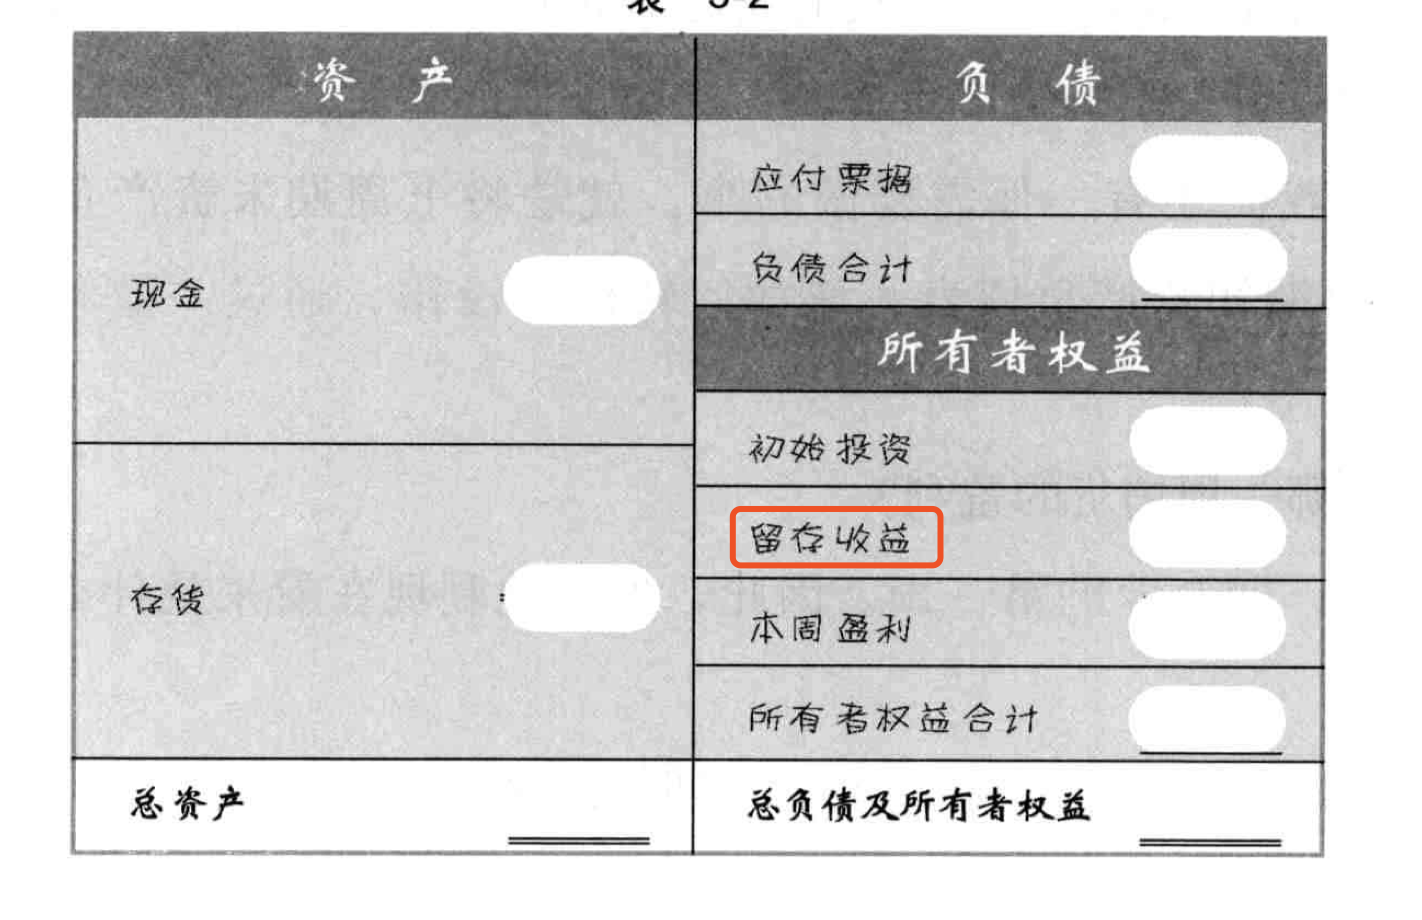
\includegraphics[width=1\textwidth]{fig/accounting_3.png}
\end{figure}

新的周期开始时,为了将我们的上期期末资产负债表更新至本期期初资产负债表,需要滚存利润,并将它们留在公司里,并将期末存货改为期初存货。

增加了应付账款的资产负债表:
\begin{figure}[H]
    \centering
    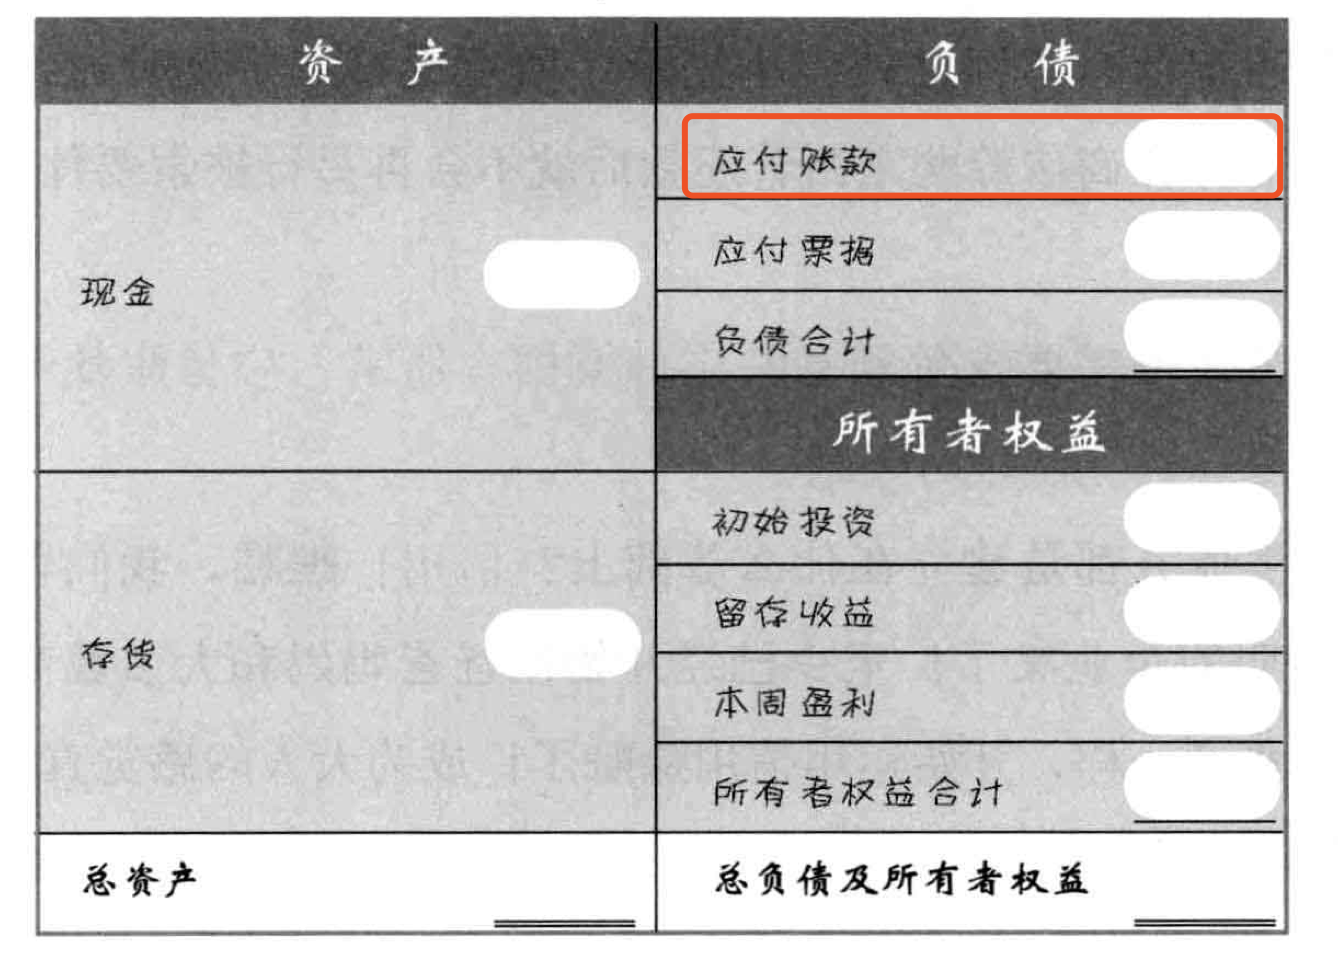
\includegraphics[width=1\textwidth]{fig/accounting_4.png}
\end{figure}

应付账款和应付票据的区别:向银行借款儿产生的应付票据说明银行贷给了你现金;杂货店的应付账款说明杂货店给了白糖,或者说存货。所以:
\begin{itemize}
\setlength{\itemsep}{0pt}
\setlength{\parsep}{0pt}
\setlength{\parskip}{0pt}
    \item 应付票据因收到他人的借款而产生;因应付票据获得现金。
    \item 应付账款因赊账购买原材料等物品而产生;因应付账款获得商品或服务。
\end{itemize}

另外,二者时间上的要求不同,一般而言,应付票据的还款期限长,可能会长达几年;应付账款的还款期限短,通常是30天。负债项目通常会根据各种各类债务到期的期限长短来列式。

二者还有一点重要的区别:应付票据需要支付利息;通常应付账款不需要支付利息,除非你无法按时还款。

这两类债务都是建立在信用的基础上。

\subsection{一些术语}
产品的生产工艺是从原材料到在产品再到产成品。

在账目上如何反应工资呢?工资使得现金减少了。工资不能计入费用,实际上,工资增加了存货的价值,因此应该从现金中减去工资,并把它加到存货上。

资产负债表中的存货可以分为原材料和产成品。
\begin{figure}[H]
    \centering
    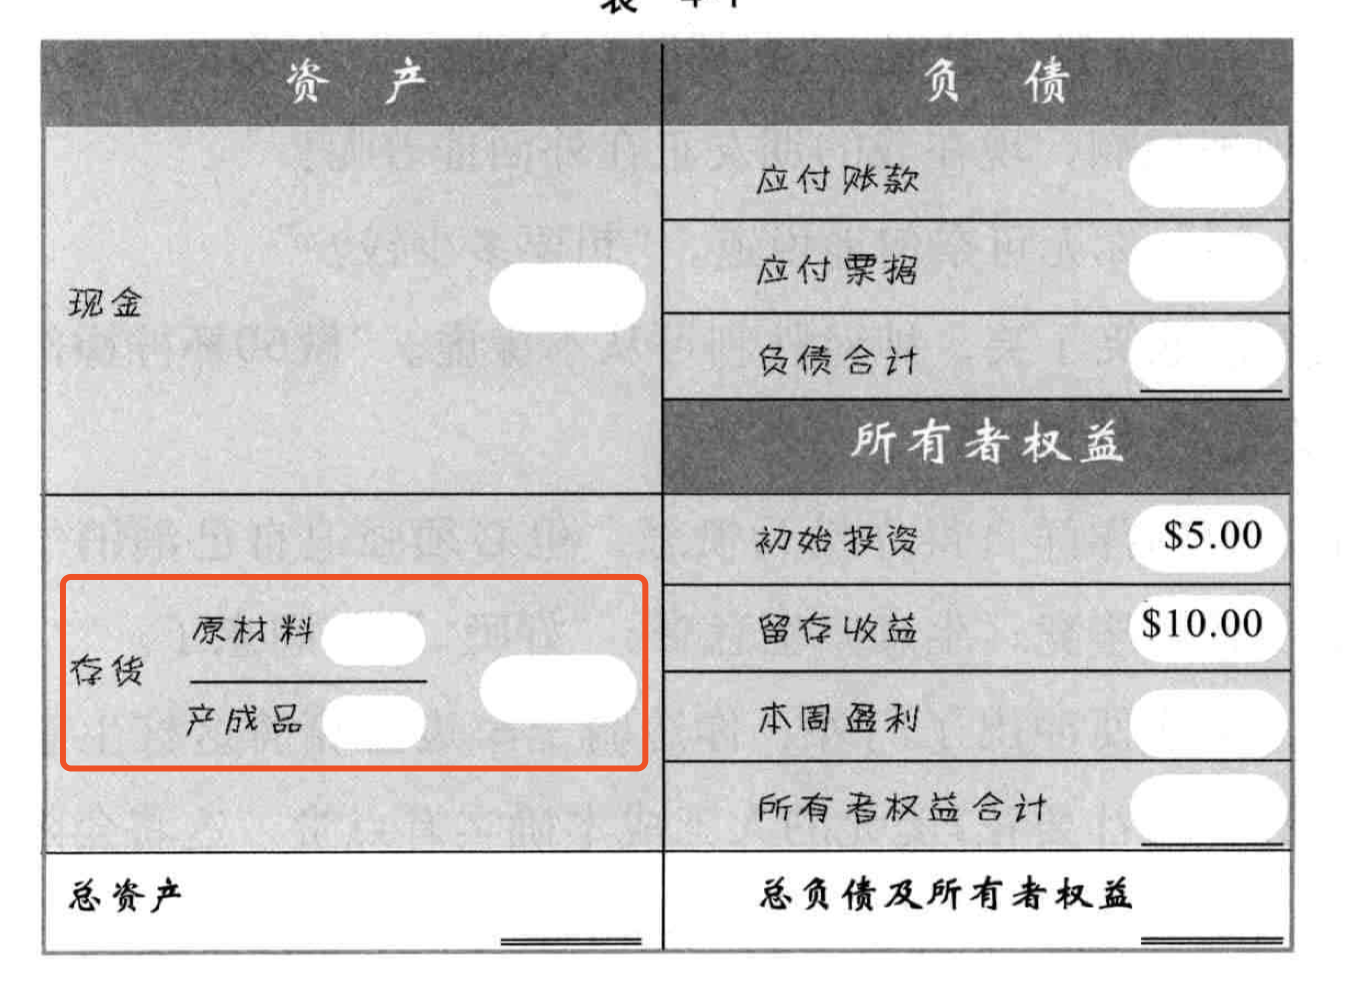
\includegraphics[width=1\textwidth]{fig/accounting_5.png}
\end{figure}

也就是说,产品制作的人工费会被捆绑在存货里面,并且将一直放在存货里,直到产品出售后才被计为费用。这也是公司通常会严控存货数量并且希望其尽快出售的原因之一。

如果是赊账出售了产品,那么在资产负债表中要增加一项为应收账款,如下:
\begin{figure}[H]
    \centering
    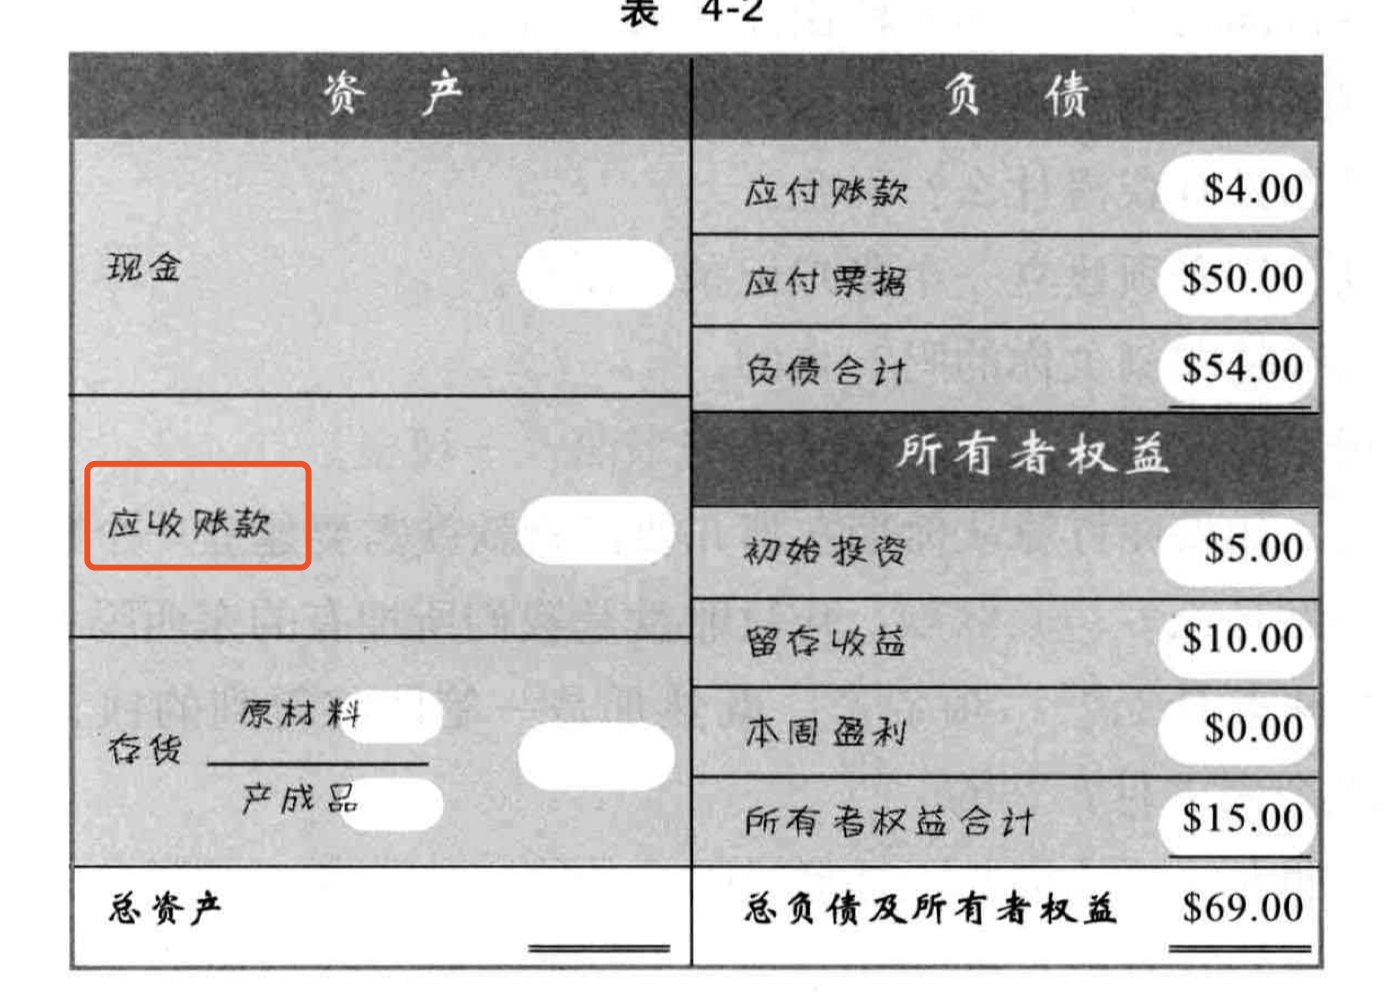
\includegraphics[width=1\textwidth]{fig/accounting_6.png}
\end{figure}

利息费用会在利润表中表示,因为它不是贷款的本金,而是贷款的成本,应该反映在利润表中。

待摊费用:预付的费用,例如一下购买的3年期保险。
\begin{figure}[H]
    \centering
    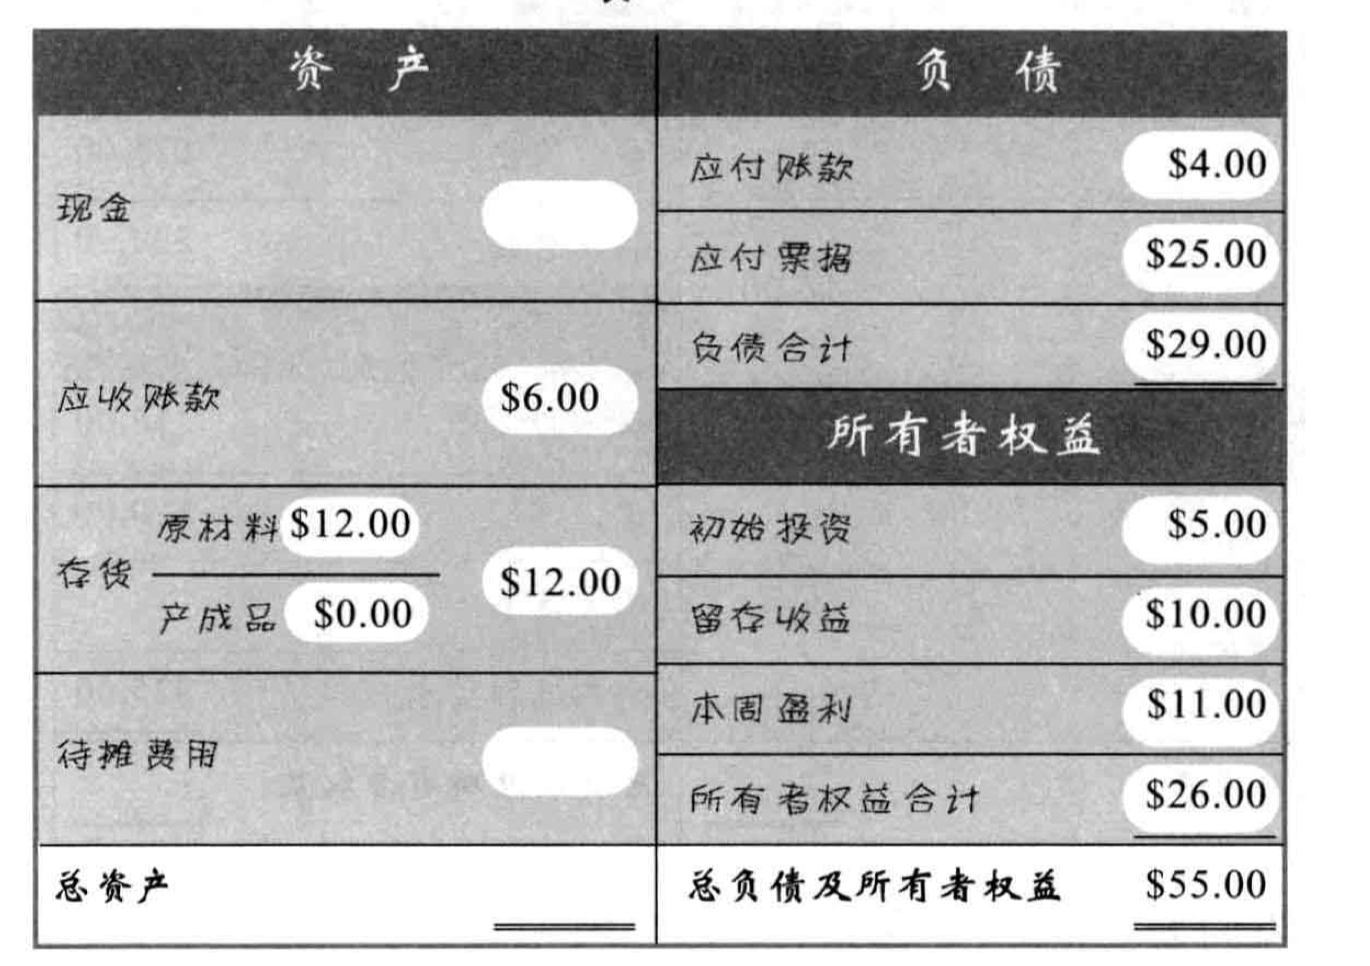
\includegraphics[width=1\textwidth]{fig/accounting_7.png}
\end{figure}

这里将费用列式为资产的原因是,当我们预付一笔费用时,它在未来的会计期间都具有价值。

回到保险的例子,我们买了保险一年后,会将其消耗掉;所以第一年的保费是一笔即期费用。做账的时候需要从中减去1元;第二年,再摊销1元;

权责发生制:将所发生的交易都进行会计核算,无论是否支付或者受到了现金。权责发生制起源于人们开始使用信用购物。商业信用产生了,购贷款可以被允许以后支付。权责发生制能够更准确地对公司的财务状况进行核算,即使现金未被收到或支付。

根据权责发生制,销售收入并不是在收到现金时才被确认,而是在能够获得权益时即确认;同理,采购发生时也要即可确认,不论是否支付了采购款。

也就是说,在权责发生制下,我们都是在交易事项的实际发生时对它们进行会计核算,而不论是否收到或支付现金。另一种核算方法是收付实现制。

在收付实现制核算方法下,交易事项以现金结算时才被记录。这种情况下,所有发生的费用都会被计入进去,比如用3元购买的保险,在收付实现制下,会记录3元的费用(而非1元的费用)。所以权责发生制的结果看起来更好,会有更多的利润。

对于拥有存货的公司,必须使用权责发生制。原因是,每年年末,当我们预测年终会盈利且要支付所得税款时,会想方设法进行避税。于是我们会用现金买入大量存货,以加大销售成本,减少利润,达到少纳税甚至不纳税的目的。而政府不希望企业这么做。没有存货的公司,例如服务行业(诊所、律师行、房产中介等)才可以使用收付实现制。

\subsection{服务业}
大多数服务业的公司将成本划分为两类:服务成本和费用。服务成本是与提供服务直接相关的支出,费用是经营公司的日常所有开支。

服务公司的利润表由如下几个项目构成:

营业收入 - 服务成本 = 毛利 - 费用 = 净利润




%\printbibliography
\bibliography{../ref}
\bibliographystyle{IEEEtran}
\end{document}
